\chapter{Resultados}\label{cap:resultados}

As \campoJanelas\ janelas dos trechos analisados chegaram completas, e o valor eficaz total da aceleração nas máquinas em operação ficou de \sinalRazaoMin\ a \sinalRazaoMax\ vezes o do sensor em repouso. Nenhuma das quatro hipóteses foi corroborada. H1 ficou \hUmVeredito, com \hUmFracaoCalandra~\% das janelas da segunda rodada da calandra marcadas pelo detector treinado na primeira, e H2, H3 e H4 foram refutadas. A menor mudança detectável na velocidade eficaz passou de \SI{0,7}{\milli\meter\per\second} em três dos cinco ensaios avaliados. Com a assinatura de desbalanceamento, a fração marcada não chegou a \SI{50}{\percent} até \SI{2,8}{\milli\meter\per\second} em nenhuma das quatro máquinas. Na base pública, o detector marcou de \hQuatroFracaoTres~\% a \hQuatroFracaoQuatro~\% das janelas com desbalanceamento real e também \hQuatroFracaoZero~\% das janelas sem desbalanceamento medidas depois da remontagem do suporte. Nas análises posteriores, com as sementes de 0 a \num{99} do detector, H1 seria corroborada com \apTresVereditoUmCorroborada\ delas e indeterminada ou refutada com as demais, e H4 seria refutada com \apTresVereditoQuatroRefutada. Em três das quatro máquinas, o escore do detector ficou abaixo do limiar mesmo com os três descritores alterados pela assinatura fora da faixa do treino.

\section{Aquisição e integridade dos dados}\label{sec:res-aquisicao}

Nos trechos analisados, a sequência das \campoLeituras\ telemetrias \campoLacunasTexto, e o resumo SHA-256 de todas as janelas conferiu na exportação. A taxa de amostragem estimada pelo transmissor ficou entre \campoTaxaMin~Hz e \campoTaxaMax~Hz, com desvio máximo de \campoDesvioTaxaMax~\% em relação a \SI{1}{\kilo\hertz}, abaixo do limite de \SI{2}{\percent} do \textit{firmware}. A intensidade do sinal recebido (RSSI) das telemetrias ficou entre \campoRssiMin~dBm e \campoRssiMax~dBm.

Em repouso sobre a mesa, a densidade de ruído do acelerômetro, média de \SIrange{20}{150}{\hertz}, foi de \ruidoDensidadeX~µg/$\sqrt{\text{Hz}}$ no eixo X, \ruidoDensidadeY~µg/$\sqrt{\text{Hz}}$ no Y e \ruidoDensidadeZ~µg/$\sqrt{\text{Hz}}$ no Z (Figura~\ref{fig:ruido}a). Os dois eixos horizontais ficaram abaixo dos \ruidoDatasheet~µg/$\sqrt{\text{Hz}}$ da folha de dados do MPU-6050 \cite{invensense2011ps}. O eixo Z, vertical sobre a mesa, tem linhas abaixo de \SI{200}{\hertz} ausentes em X e em Y, o que é compatível com vibração da mesa somada ao ruído do sensor. Acima de cerca de \SI{200}{\hertz}, a densidade diminui nos três eixos, o que é compatível com o filtro interno de banda nominal de \SI{184}{\hertz}. Em velocidade, o ruído em repouso corresponde a \ruidoVelocidade~mm/s no descritor $d_1$, mediana das janelas.

\begin{figure}[!htb]
\centering
\caption{Ruído do acelerômetro em repouso e valor eficaz em cada ensaio}\label{fig:ruido}
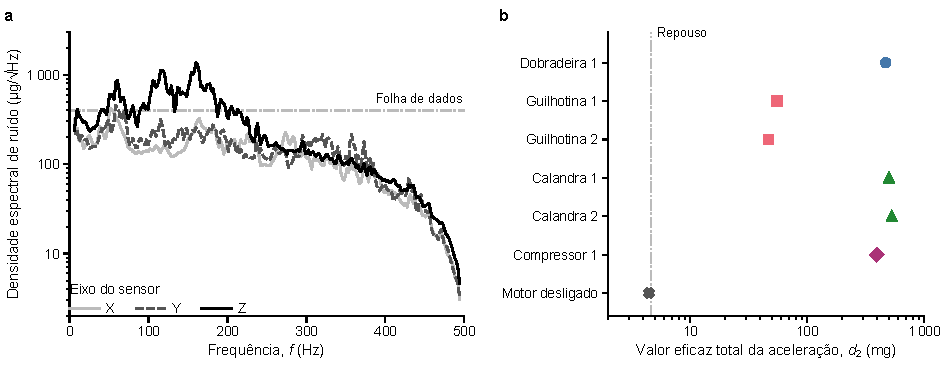
\includegraphics{fig_ruido.pdf}
\fonte{elaborado pelo próprio autor.}
\legenda{\textbf{a}, densidade espectral de ruído de cada eixo do sensor, pelo método de Welch com janela de Hann de \num{512} amostras, média das \campoJanelasRepouso\ janelas com o transmissor sobre a mesa; a linha horizontal marca os \ruidoDatasheet~µg/$\sqrt{\text{Hz}}$ da folha de dados do MPU-6050. \textbf{b}, mediana, entre as janelas de cada ensaio, do valor eficaz total da aceleração ($d_2$); o número depois do nome da máquina é a rodada, e a linha vertical marca o valor em repouso. Eixo vertical de \textbf{a} e eixo horizontal de \textbf{b} em escala logarítmica.}
\end{figure}

O valor eficaz total da aceleração, mediana das janelas de cada ensaio, foi de \sinalRmsGuilhotinaDois~mg a \sinalRmsCalandraDois~mg nas máquinas em operação, contra \ruidoRmsTotal~mg em repouso (Figura~\ref{fig:ruido}b). A guilhotina teve o menor valor, de \sinalRazaoGuilhotinaDois\ a \sinalRazaoGuilhotinaUm\ vezes o de repouso. No trecho com o motor desligado, o valor foi de \sinalRmsMotorParadoDecimal~mg, \sinalRazaoMotorParadoDecimal\ vez o de repouso.

Das \reiniciosInicio\ às \reiniciosFim, o transmissor reiniciou por queda de tensão da bateria, e esse intervalo é chamado aqui de período de reinícios. O período começa com as primeiras reinicializações e termina na hora da última das \rajadasSequenciaUmPeriodo\ rajadas enviadas no primeiro ciclo depois de uma inicialização. Fora dele, \rajadasForaCompletas\ das \rajadasFora\ rajadas do histórico de eventos do \textit{gateway} chegaram completas (\rajadasForaPct~\%), isto é, com os \num{26} fragmentos depois de no máximo três tentativas. A rajada completa durou \rajadasDuracaoMediana~s, mediana entre elas. A fração de rajadas completas variou com a RSSI da telemetria do mesmo ciclo (Figura~\ref{fig:enlace}). Com RSSI de \SI{-80}{dBm} ou mais, \rajadasAcimaOitentaPct~\% chegaram completas, de \SI{-110}{dBm} a \SI{-80}{dBm}, \rajadasCentoDezOitentaCompletas\ das \rajadasCentoDezOitenta, e abaixo de \SI{-110}{dBm}, \rajadasAbaixoCentoDezCompletas\ de \rajadasAbaixoCentoDez. Como a posição do transmissor e do \textit{gateway} em cada rajada não foi anotada, os dados não permitem atribuir à distância a variação da RSSI.

Das \rajadasFalhasTotal\ rajadas incompletas registradas no histórico de 2 de novembro, \rajadasFalhasReinicio\ ocorreram durante o período de reinícios. Das \rajadasForaIncompletas\ fora desse período, \rajadasForaSemFragmento\ não tiveram nenhum fragmento recebido. Nenhuma rajada incompleta ocorreu nos trechos analisados, e nenhuma janela desses trechos ficou com fragmento ausente.

\begin{figure}[!htb]
\centering
\caption{Rajadas completas em função da intensidade do sinal recebido}\label{fig:enlace}
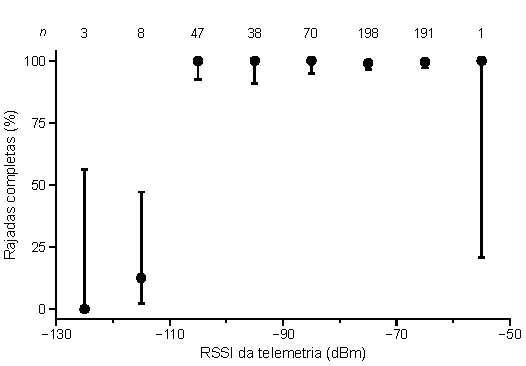
\includegraphics{fig_enlace.pdf}
\fonte{elaborado pelo próprio autor.}
\legenda{fração das rajadas do histórico de eventos do \textit{gateway} que chegaram com os \num{26} fragmentos, depois de no máximo três tentativas, em faixas de \SI{10}{dB} da RSSI da telemetria do mesmo ciclo, com o ponto no centro da faixa. As barras mostram o intervalo de confiança de \SI{95}{\percent} de \citeonline{wilson1927}, e $n$, acima do gráfico, é o número de rajadas da faixa. Exclui o período de reinícios por bateria, das \reiniciosInicio\ às \reiniciosFim.}
\end{figure}

\section{Linha de base das máquinas}\label{sec:res-base}

A rotação estimada na dobradeira, na guilhotina e na calandra ficou entre \rotacaoRpmMin\ e \rotacaoRpmMax~r/min, perto da velocidade síncrona de \SI{1800}{r/min} de um motor de quatro polos em \SI{60}{\hertz}, e a do compressor, em \rotacaoRpmCompressorUm~r/min, perto dos \SI{3600}{r/min} de um motor de dois polos. Só a guilhotina e a calandra têm placa legível, e o número de polos da dobradeira e do compressor é uma suposição (seção~\ref{sec:descritores}). Na guilhotina e na calandra, a rotação ficou acima da nominal de placa, de \SI{1760}{r/min} e \SI{1715}{r/min}, o que é compatível com a operação sem carga, em que o escorregamento é menor que o nominal \cite{chapman2012}. Entre as janelas de um mesmo ensaio, a rotação estimada teve desvio-padrão de \rotacaoDesvioMin~Hz a \rotacaoDesvioMax~Hz, ou de \rotacaoDesvioPctMin~\% a \rotacaoDesvioPctMax~\% da velocidade síncrona. Pela mediana das janelas, o escorregamento estimado foi de no máximo \escorregamentoCalandraDois~\%, na segunda rodada da calandra, e de \escorregamentoGuilhotinaDois~\% na segunda rodada da guilhotina, com a rotação acima da síncrona por menos que o desvio-padrão entre janelas de qualquer ensaio.

Nos espectros médios dos seis ensaios, \picosTotal\ linhas ficaram acima de dez vezes o nível mediano do espectro, \picosPrimeiraRodada\ delas nos ensaios da primeira rodada, mostrados na Figura~\ref{fig:espectros}. Uma linha foi associada a uma ordem da rotação quando ficou a até \picosTolerancia~Hz dela. Das \picosTotal\ linhas, \picosDiretos\ coincidem com ordens da rotação, \picosRebatidos\ coincidem com ordens acima de \SI{500}{\hertz} rebatidas pela amostragem a \SI{1}{\kilo\hertz} (equação do rebatimento, seção~\ref{sec:fund-aquisicao}) e \picosNaoIdentificados\ não foram associadas a uma ordem. As ordens rebatidas estão na guilhotina, \picosRebatidosGuilhotinaUm\ na primeira rodada (Figura~\ref{fig:espectros}b) e \picosRebatidosGuilhotinaDois\ na segunda, fora da figura. As linhas rebatidas são compatíveis com conteúdo acima de \SI{500}{\hertz} rebatido na amostragem, apesar do filtro interno de \SI{184}{\hertz}, que é digital \cite{invensense2012rm}.

\begin{figure}[!htb]
\centering
\caption{Espectro médio da aceleração na primeira rodada de cada máquina}\label{fig:espectros}
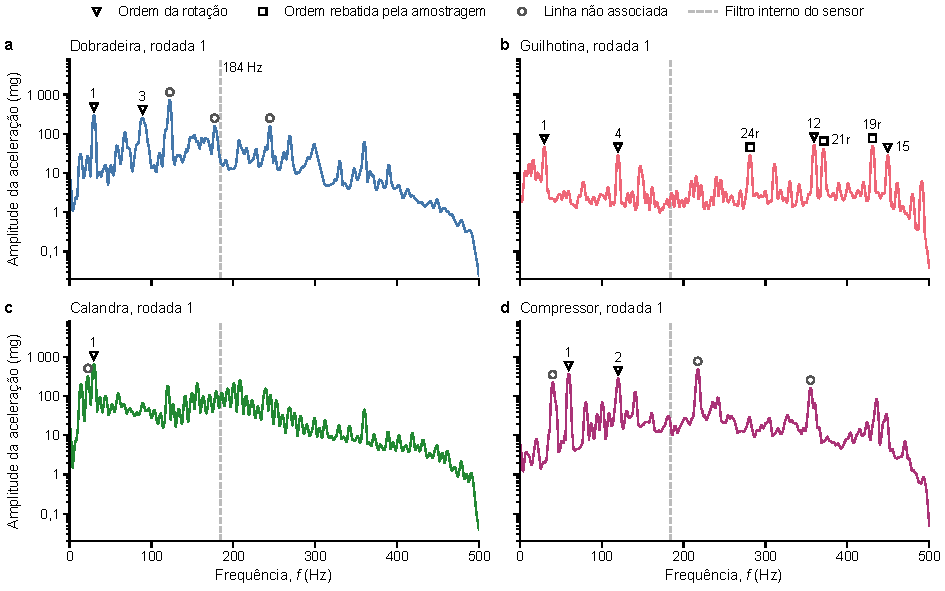
\includegraphics{fig_espectros.pdf}
\fonte{elaborado pelo próprio autor.}
\legenda{amplitude da aceleração com os três eixos somados, média das janelas do ensaio, com janela de Hann e preenchimento com zeros até quatro vezes o tamanho da janela; eixo vertical em escala logarítmica, comum aos quatro painéis. Os marcadores ficam sobre as linhas acima de dez vezes o nível mediano do espectro. Uma linha foi associada a uma ordem da rotação quando ficou a até \picosTolerancia~Hz dela, e o número junto ao marcador é a ordem, seguido de r quando a ordem passa de \SI{500}{\hertz} e aparece rebatida pela amostragem. A linha vertical marca a banda nominal de \SI{184}{\hertz} do filtro interno do sensor. \textbf{a}, dobradeira; \textbf{b}, guilhotina; \textbf{c}, calandra; \textbf{d}, compressor.}
\end{figure}

A velocidade eficaz de \SIrange{10}{184}{\hertz} foi maior na direção axial do que nas radiais na dobradeira, na calandra e no compressor, com medianas de \velAxialDobradeiraUm, \velAxialCalandraUm\ e \velAxialCompressorUm~mm/s (Figura~\ref{fig:eixos}). Na guilhotina, a direção axial teve o menor valor, e a maior velocidade, radial, teve mediana de \velMaxGuilhotinaUm~mm/s. As três medianas axiais passam do limite entre as zonas C e D do grupo 2 em fundação rígida, de \SI{4,5}{\milli\meter\per\second}, e as da dobradeira e da calandra passam também o de fundação flexível, de \SI{7,1}{\milli\meter\per\second} \cite{iso208163_2022}. Como a faixa de \SIrange{10}{184}{\hertz} está contida na de \SIrange{10}{1000}{\hertz} da norma, esses valores são limites inferiores da velocidade eficaz de banda larga no mesmo sinal. O sinal, porém, é o medido pelo transmissor depois da fita, do invólucro e das espumas, e a resposta dessa fixação não foi medida (seção~\ref{sec:ensaios}).

\begin{figure}[!htb]
\centering
\caption{Velocidade eficaz por direção em cada ensaio}\label{fig:eixos}
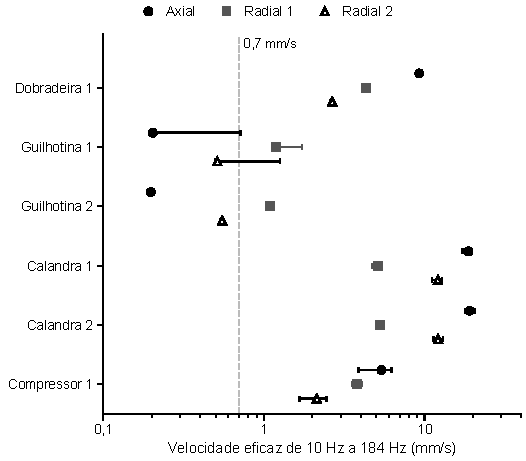
\includegraphics{fig_eixos.pdf}
\fonte{elaborado pelo próprio autor.}
\legenda{mediana (marcador) e intervalo interquartil (barra), entre as janelas de cada ensaio, da velocidade eficaz de \SIrange{10}{184}{\hertz} em cada eixo do sensor, identificado pela direção em relação ao eixo do motor; o número depois do nome da máquina é a rodada. A linha vertical marca o tamanho de referência de \SI{0,7}{\milli\meter\per\second} (seção~\ref{sec:hipoteses}). Eixo horizontal em escala logarítmica.}
\end{figure}

\section{Falso alarme entre rodadas}\label{sec:res-h1}

Treinado na primeira rodada, o detector principal marcou \hUmCalandraIFDireto~\% das janelas da segunda rodada da calandra, com intervalo de confiança de \SI{95}{\percent} de \hUmCalandraIFDiretoInf~\% a \hUmCalandraIFDiretoSup~\%, e \hUmGuilhotinaIFDireto~\% das janelas da segunda rodada da guilhotina. Na calandra, a fração ficou acima dos \SI{10}{\percent} do critério de corroboração e abaixo dos \SI{20}{\percent} do critério de refutação, e H1 ficou \hUmVeredito. O intervalo registrado reamostra só as janelas de teste. Com as sementes de 0 a \num{99} do detector, a fração marcada na calandra teve mediana de \apTresSementeCalandraMed~\%, abaixo dos \hUmFracaoCalandra~\% da semente 0, registrada, e H1 seria corroborada com \apTresVereditoUmCorroborada\ das \apTresSementes\ sementes (seção~\ref{sec:res-ap3}).

Entre as duas rodadas da calandra, várias condições da medição mudaram ao mesmo tempo. O transmissor foi colado de novo, com fita nova, a alimentação passou da bateria para o carregador portátil, e o intervalo entre ciclos passou de \campoCicloUm\ para \campoCicloDois~s. A temperatura do sensor, mediana da telemetria, passou de \campoTempCalandraUm\ para \campoTempCalandraDois~\si{\celsius}, e os inícios dos dois ensaios ficaram separados por \campoIntervaloCalandra. A mediana de $d_1$ variou \repetCalandraDif~\%, de \repetCalandraUm\ para \repetCalandraDois~mm/s. Na guilhotina, a fixação, a alimentação e o ciclo mudaram da mesma forma, a temperatura passou de \campoTempGuilhotinaUm\ para \campoTempGuilhotinaDois~\si{\celsius}, a mediana de $d_1$ variou \repetGuilhotinaDif~\%, de \repetGuilhotinaUm\ para \repetGuilhotinaDois~mm/s, e o sensor ficou invertido de uma rodada para a outra (seção~\ref{sec:ensaios}). Os dados não separam o efeito de cada uma dessas mudanças sobre a fração marcada.

No sentido inverso, com treino na segunda rodada, o detector principal marcou \hUmCalandraIFInverso~\% das janelas da primeira rodada da calandra e \hUmGuilhotinaIFInverso~\% das da guilhotina, que tem só \campoJanelasGuilhotinaUm\ janelas nessa rodada. A regra por mediana e MAD não marcou nenhuma janela no sentido direto e marcou \hUmCalandraMADInverso~\% e \hUmGuilhotinaMADInverso~\% no inverso. Os resultados do sentido inverso e da regra por MAD são descritivos e não entram no critério.

\section{Menor mudança detectável}\label{sec:res-h2}

A menor mudança detectável no descritor $d_1$ ficou abaixo de \SI{0,7}{\milli\meter\per\second} na dobradeira e na segunda rodada da guilhotina e acima desse valor no compressor e nas duas rodadas da calandra (Tabela~\ref{tab:h2}). Pelo critério registrado, H2 foi refutada. A menor mudança detectável não acompanhou o nível de $d_1$. A dobradeira, com mediana de \hDoisMedianaDobradeiraUm~mm/s, teve menor mudança detectável de \hDoisMmdDobradeiraUm~mm/s, e o compressor, com mediana de \hDoisMedianaCompressorUm~mm/s, de \hDoisMmdCompressorUm~mm/s.

\begin{table}[!htb]
\centering\small
\caption{Menor mudança detectável no descritor $d_1$ em cada ensaio da coleta de 2 de novembro de 2026}\label{tab:h2}
\begin{tabular}{@{}llrrrrr@{}}
\toprule
Máquina & Rodada & Janelas & Mediana & Quantil de \SI{95}{\percent} & \multicolumn{2}{c}{Menor mudança detectável} \\
\cmidrule(l){6-7}
 & & & (mm/s) & (mm/s) & (mm/s) & (\%) \\
\midrule
Dobradeira & 1 & \hDoisNDobradeiraUm & \hDoisMedianaDobradeiraUm & \hDoisQDobradeiraUm & \hDoisMmdDobradeiraUm & \hDoisRelDobradeiraUm \\
Guilhotina & 1 & \hDoisNGuilhotinaUm & \hDoisMedianaGuilhotinaUm & \hDoisQGuilhotinaUm & \hDoisMmdGuilhotinaUm & \hDoisRelGuilhotinaUm \\
Guilhotina & 2 & \hDoisNGuilhotinaDois & \hDoisMedianaGuilhotinaDois & \hDoisQGuilhotinaDois & \hDoisMmdGuilhotinaDois & \hDoisRelGuilhotinaDois \\
Calandra & 1 & \hDoisNCalandraUm & \hDoisMedianaCalandraUm & \hDoisQCalandraUm & \hDoisMmdCalandraUm & \hDoisRelCalandraUm \\
Calandra & 2 & \hDoisNCalandraDois & \hDoisMedianaCalandraDois & \hDoisQCalandraDois & \hDoisMmdCalandraDois & \hDoisRelCalandraDois \\
Compressor & 1 & \hDoisNCompressorUm & \hDoisMedianaCompressorUm & \hDoisQCompressorUm & \hDoisMmdCompressorUm & \hDoisRelCompressorUm \\
\bottomrule
\end{tabular}
\fonte{elaborada pelo próprio autor.}
\nota{a menor mudança detectável é a diferença entre o quantil de \SI{95}{\percent} e a mediana de $d_1$ no ensaio; em porcentagem, relativa à mediana. A primeira rodada da guilhotina, com menos de \num{25} janelas, não entra no critério de H2.}
\end{table}

A refutação de H2 não depende de poucas janelas. Na reamostragem por blocos da AP4, todas as réplicas das duas rodadas da calandra e do compressor ficaram acima de \SI{0,7}{\milli\meter\per\second}, e a menor mudança detectável da segunda rodada da guilhotina, abaixo desse valor na amostra, passou dele em \apQuatroAcimaGuilhotinaDois~\% das réplicas (seção~\ref{sec:res-ap4}). Pela mesma regra, a menor mudança detectável de $d_1$ com o sensor em repouso foi de \apCincoMmd~mm/s, e a dos cinco ensaios do critério ficou de \apCincoRazaoMin\ a \apCincoRazaoMax\ vezes esse valor (seção~\ref{sec:res-ap5}). A variação de $d_1$ entre janelas nas máquinas foi, portanto, maior que a do sensor parado. Ela reúne a vibração da máquina e a resposta da fixação do transmissor, e os dados não separam as duas.

A primeira rodada da guilhotina, que não entra no critério, teve a maior variação relativa, com quantil de \SI{95}{\percent} de \hDoisQGuilhotinaUm~mm/s para uma mediana de \hDoisMedianaGuilhotinaUm~mm/s. Os acionamentos da lâmina durante os ensaios não foram anotados, e os dados não permitem dizer se as janelas com $d_1$ mais alto coincidem com eles.

\section{Detecção das assinaturas injetadas}\label{sec:res-h3}

Com o detector principal, a fração marcada não chegou a \SI{50}{\percent} em nenhuma máquina até \SI{2,8}{\milli\meter\per\second} de assinatura em cada eixo radial (Figura~\ref{fig:injecao}). Entre todas as amplitudes da grade, a maior fração marcada foi de \hTresFracaoMaxCalandra~\% na calandra, \hTresFracaoMaxDobradeira~\% na dobradeira, \hTresFracaoMaxGuilhotina~\% na guilhotina e \hTresFracaoMaxCompressor~\% no compressor. Pelo critério registrado, H3 foi refutada.

A correlação de Spearman entre a amplitude e a fração marcada foi de \hTresRhoDobradeira\ na dobradeira, \hTresRhoGuilhotina\ na guilhotina, \hTresRhoCalandra\ na calandra e \hTresRhoCompressor\ no compressor. Na dobradeira e no compressor, as janelas marcadas foram de \hTresJanelasMinDobradeira\ a \hTresJanelasMaxDobradeira\ das \hTresTesteDobradeira\ janelas de teste e de \hTresJanelasMinCompressor\ a \hTresJanelasMaxCompressor\ das \hTresTesteCompressor\ em toda a grade de amplitudes, e as correlações negativas refletem a oscilação dessas poucas janelas.

Nenhuma das dez florestas de cada máquina, treinadas com as sementes de 0 a 9 do gerador de números aleatórios, chegou a \SI{50}{\percent} de janelas marcadas. A regra por mediana e MAD, que sem assinatura já marcava \hTresMadZeroDobradeira~\% das janelas de teste da dobradeira, chegou a \SI{50}{\percent} só nessa máquina, com \hTresMadDobradeira~mm/s. A assinatura do dobro da rotação no eixo axial, calculada como descrição, chegou a \SI{50}{\percent} só na guilhotina, com \hTresDoisXGuilhotina~mm/s.

\begin{figure}[!htb]
\centering
\caption{Fração de janelas marcadas em função da amplitude da assinatura de desbalanceamento}\label{fig:injecao}
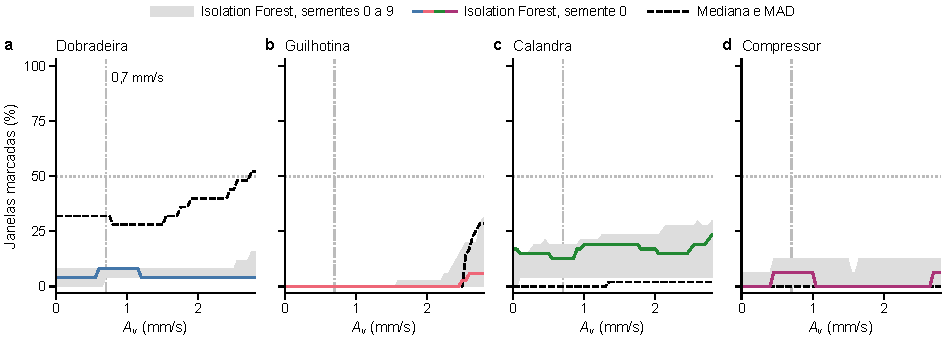
\includegraphics{fig_injecao.pdf}
\fonte{elaborado pelo próprio autor.}
\legenda{assinatura na rotação somada aos dois eixos radiais em quadratura, com velocidade eficaz $A_v$ em cada eixo, às janelas de teste da dobradeira (\textbf{a}, \hTresTesteDobradeira\ janelas), da guilhotina (\textbf{b}, \hTresTesteGuilhotina), da calandra (\textbf{c}, \hTresTesteCalandra) e do compressor (\textbf{d}, \hTresTesteCompressor). A floresta com semente 0 é o detector do critério; a faixa vai do mínimo ao máximo das dez florestas treinadas com as sementes de 0 a 9 do gerador de números aleatórios. A linha horizontal marca os \SI{50}{\percent} que definem $A_{50}$, e a vertical, o tamanho de referência de \SI{0,7}{\milli\meter\per\second}.}
\end{figure}

Antes da injeção, a componente na rotação, $d_5$, tinha mediana de \hTresBaseUmXDobradeira~mm/s nas janelas de teste da dobradeira e de \hTresBaseUmXCalandra~mm/s nas da calandra, contra \hTresBaseUmXGuilhotina~mm/s na guilhotina e \hTresBaseUmXCompressor~mm/s no compressor. Somados em quadratura nos dois eixos radiais, os \SI{2,8}{\milli\meter\per\second} de assinatura em cada eixo correspondem a \SI{4,0}{\milli\meter\per\second} em $d_5$, menos que a componente já presente na dobradeira e na calandra.

Na guilhotina e no compressor, a assinatura de \SI{2,8}{\milli\meter\per\second} elevou os escores das janelas de teste, e só os maiores passaram do limiar. O treino teve \hTresTreinoGuilhotina\ e \hTresTreinoCompressor\ janelas, e o limiar ficou em \hTresLimiarGuilhotina\ na guilhotina e \hTresLimiarCompressor\ no compressor. Sem assinatura, os escores das janelas de teste foram de \hTresEscoreZeroMinGuilhotina\ a \hTresEscoreZeroMaxGuilhotina\ e de \hTresEscoreZeroMinCompressor\ a \hTresEscoreZeroMaxCompressor, e com \SI{2,8}{\milli\meter\per\second}, de \hTresEscoreAltoMinGuilhotina\ a \hTresEscoreAltoMaxGuilhotina\ e de \hTresEscoreAltoMinCompressor\ a \hTresEscoreAltoMaxCompressor. Nessas duas máquinas, o escore de um ponto com $d_1$, $d_2$ e $d_5$ acima da faixa do treino e os demais descritores na mediana do treino fica abaixo do limiar (seção~\ref{sec:res-ap6}).

\section{Aplicação do detector principal a outras máquinas e ao motor desligado}\label{sec:res-condicao}

Como descrição, o detector principal treinado em cada máquina foi aplicado às janelas de teste das outras máquinas e ao trecho com o motor desligado. Treinado na dobradeira, na guilhotina ou na calandra, ele marcou todas as janelas das outras máquinas, com uma exceção: o modelo da dobradeira marcou \condDobradeiraCalandra~\% das janelas da calandra. Treinado no compressor, marcou \condCompressorDobradeira~\% das janelas da dobradeira, \condCompressorGuilhotina~\% das da guilhotina e \condCompressorCalandra~\% das da calandra. O motor desligado foi marcado em \condDobradeiraParado~\% e \condCalandraParado~\% das janelas pelos modelos da dobradeira e da calandra, em \condCompressorParado~\% pelo do compressor e em \condGuilhotinaParado~\% pelo da guilhotina.

\section{Desbalanceamento real na base pública}\label{sec:res-h4}

Com treino nas \hQuatroNTreino\ janelas de 0D, o detector principal marcou \hQuatroFracaoZero~\% das \hQuatroNZero\ janelas de 0E, sem desbalanceamento, com intervalo de confiança de \SI{95}{\percent} de \hQuatroIcInfZero~\% a \hQuatroIcSupZero~\% (Tabela~\ref{tab:h4}). Nos quatro níveis de desbalanceamento, marcou de \hQuatroFracaoTres~\% a \hQuatroFracaoQuatro~\% das janelas, e o menor nível com \SI{50}{\percent} ou mais foi o \hQuatroMenorNivel. Como o falso alarme em 0E passou dos \SI{20}{\percent} do critério de refutação, H4 foi \hQuatroVeredito.

\begin{table}[!htb]
\centering\small
\caption{Frações de janelas marcadas na base pública de desbalanceamento}\label{tab:h4}
\setlength{\tabcolsep}{4pt}
\begin{tabular}{@{}lcrrrrrrr@{}}
\toprule
Arquivo & Nível & Janelas & \multicolumn{2}{c}{Detector principal (\%)} & MAD & Banda & \textit{Vibration\_1} & Mediana \\
\cmidrule(lr){4-5}
 & & & Fração & Intervalo de \SI{95}{\percent} & (\%) & completa (\%) & (\%) & de $d_5$ \\
\midrule
0D & 0 & \hQuatroNTreino & & & & & & \hQuatroDcincoMedianaTreino \\
0E & 0 & \hQuatroNZero & \hQuatroFracaoZero & \hQuatroIcInfZero\ a \hQuatroIcSupZero & \hQuatroFracaoMadZero & \hQuatroFracaoBandaCompletaZero & \hQuatroFracaoVibUmZero & \hQuatroDcincoMedianaZero \\
1E & 1 & \hQuatroNUm & \hQuatroFracaoUm & \hQuatroIcInfUm\ a \hQuatroIcSupUm & \hQuatroFracaoMadUm & \hQuatroFracaoBandaCompletaUm & \hQuatroFracaoVibUmUm & \hQuatroDcincoMedianaUm \\
2E & 2 & \hQuatroNDois & \hQuatroFracaoDois & \hQuatroIcInfDois\ a \hQuatroIcSupDois & \hQuatroFracaoMadDois & \hQuatroFracaoBandaCompletaDois & \hQuatroFracaoVibUmDois & \hQuatroDcincoMedianaDois \\
3E & 3 & \hQuatroNTres & \hQuatroFracaoTres & \hQuatroIcInfTres\ a \hQuatroIcSupTres & \hQuatroFracaoMadTres & \hQuatroFracaoBandaCompletaTres & \hQuatroFracaoVibUmTres & \hQuatroDcincoMedianaTres \\
4E & 4 & \hQuatroNQuatro & \hQuatroFracaoQuatro & \hQuatroIcInfQuatro\ a \hQuatroIcSupQuatro & \hQuatroFracaoMadQuatro & \hQuatroFracaoBandaCompletaQuatro & \hQuatroFracaoVibUmQuatro & \hQuatroDcincoMedianaQuatro \\
\bottomrule
\end{tabular}
\fonte{elaborada pelo próprio autor, com dados de \citeonline{mey2022dados}.}
\nota{0D é o arquivo de treino, e 0E a 4E, os de avaliação, medidos depois da remontagem do suporte. Os níveis 1 a 4 têm desbalanceamento de \SIlist{45,9;60,7;75,5;152,1}{\milli\meter\gram} (seção~\ref{sec:base-publica}). O detector principal é o Isolation Forest da seção~\ref{sec:detectores}; MAD é a regra por mediana e MAD; banda completa, o detector principal com $d_2$ a $d_4$ sem o corte em \SI{184}{\hertz} e $d_1$ de \SIrange{10}{1000}{\hertz}; \textit{Vibration\_1}, o detector principal só com o canal usado pelos autores da base. As três últimas frações são descritivas. $d_5$ está na unidade dos canais, que a base não informa.}
\end{table}

O falso alarme acompanhou uma mudança do sinal entre os dois arquivos sem desbalanceamento (Figura~\ref{fig:h4}). De 0D para 0E, a mediana de $d_1$ passou de \hQuatroDumMedianaTreino\ para \hQuatroDumMedianaZero, e a de $d_5$, de \hQuatroDcincoMedianaTreino\ para \hQuatroDcincoMedianaZero, na unidade dos canais. Entre essas duas medições, o suporte do desbalanceamento foi desmontado e remontado (seção~\ref{sec:base-publica}). A mudança é compatível com o efeito da remontagem, e os dados não permitem separá-la de outras diferenças entre as duas medições.

No nível 1, a mediana de $d_5$, de \hQuatroDcincoMedianaUm, ficou próxima da de 0E, e o detector marcou \hQuatroFracaoUm~\% das janelas. Em 1E, a curtose ($d_3$) teve mediana de \hQuatroDtresMedianaUm, contra \hQuatroDtresMedianaZero\ em 0E, e o fator de crista ($d_4$), de \hQuatroDquatroMedianaUm, contra \hQuatroDquatroMedianaZero. A curtose e o fator de crista mais altos indicam componentes impulsivas que os outros arquivos não têm, e os dados não permitem atribuir ao desbalanceamento a marcação do nível 1.

Do nível 2 ao 4, a mediana de $d_5$ cresceu com o desbalanceamento, de \hQuatroDcincoMedianaDois\ para \hQuatroDcincoMedianaQuatro, e a de $d_1$, de \hQuatroDumMedianaDois\ para \hQuatroDumMedianaQuatro. A fração marcada não seguiu essa ordem, com \hQuatroFracaoDois~\% no nível 2, \hQuatroFracaoTres~\% no 3 e \hQuatroFracaoQuatro~\% no 4, e a correlação de Spearman entre o desbalanceamento e a fração marcada foi de \hQuatroRho.

\begin{figure}[!htb]
\centering
\caption{Escore do detector, velocidade eficaz e curtose em cada arquivo da base pública}\label{fig:h4}
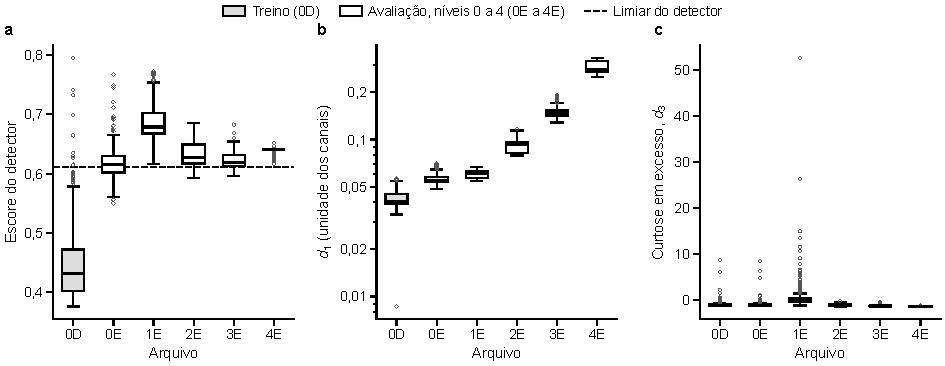
\includegraphics{fig_h4.pdf}
\fonte{elaborado pelo próprio autor, com dados de \citeonline{mey2022dados}.}
\legenda{distribuição, entre as janelas de cada arquivo da base pública, do escore do detector principal (\textbf{a}), de $d_1$ (\textbf{b}) e da curtose em excesso, $d_3$ (\textbf{c}). 0D é o arquivo de treino, e 0E a 4E, os de avaliação, com os níveis de desbalanceamento 0 a 4. A caixa vai do primeiro ao terceiro quartil, a linha interna marca a mediana, as hastes vão até 1,5 vez o intervalo interquartil, e os círculos são os valores além delas. Em \textbf{a}, a linha horizontal marca o limiar do detector, estimado no treino; em \textbf{b}, o eixo vertical está em escala logarítmica e na unidade dos canais, que a base não informa.}
\end{figure}

Com as sementes 0 a 9, previstas como descrição no registro de H4, o falso alarme em 0E variou de \hQuatroFaSementeMin~\% a \hQuatroFaSementeMax~\%, e a seção~\ref{sec:res-ap3} amplia essa variação para as sementes 0 a 99. A regra por mediana e MAD marcou \hQuatroFracaoMadZero~\% das janelas de 0E. Com a banda completa, o falso alarme foi de \hQuatroFracaoBandaCompletaZero~\%, e a fração marcada no nível 3 ficou em \hQuatroFracaoBandaCompletaTres~\%. Em nenhuma das variantes calculadas com a semente 0, o falso alarme ficou dentro dos \SI{10}{\percent} do critério de corroboração.

\section{Análises posteriores}\label{sec:res-posteriores}

Duas emendas ao registro acrescentaram seis análises posteriores, cada uma com o procedimento definido antes do cálculo (Apêndice~\ref{ap:registro}). A AP1 e a AP2, de 7 de novembro de 2026, examinam os resultados de H3 e de H2. A AP3 a AP6, de 8 de novembro, foram pedidas por pareceres sobre uma versão anterior deste texto e tratam da incerteza de H1, H2 e H4 e do escore do detector principal. Só a AP1 tem previsão registrada. As emendas mantiveram os critérios de H1 a H4, e as seis análises não alteram a avaliação dessas hipóteses.

\subsection{Assinatura em fase com a componente na rotação}\label{sec:res-ap1}

Em H3, a fase da assinatura foi sorteada em cada janela. Como o início da janela não é sincronizado com o eixo, a diferença de fase entre a assinatura e a componente na rotação já presente no sinal também variou ao acaso de uma janela para outra. Em um desbalanceamento real, a força acrescentada tem fase fixa em relação à do desbalanceamento existente, porque a massa fica em um ponto do rotor, e, com resposta linear da estrutura, essa diferença de fase é a mesma em todos os eixos. Na AP1, a componente na rotação já presente no sinal foi atribuída a desbalanceamento. Se parte dela tiver outra origem, como desalinhamento ou folga, a diferença de fase entre um desbalanceamento real e essa componente não será a mesma em todos os eixos.

A fase da componente na rotação de cada eixo radial foi medida em cada janela de teste, pelo coeficiente da transformada de Fourier da janela na frequência de rotação. A assinatura foi somada com diferença de fase $\theta$ de \SI{0}{\degree}, \SI{90}{\degree} ou \SI{180}{\degree} em relação a essa componente. As máquinas, a divisão entre treino e teste, o detector, o limiar e a grade de amplitudes foram os de H3, e a injeção foi conferida antes do cálculo em uma janela sintética com fase conhecida.

A previsão registrada era que, com $\theta = \SI{0}{\degree}$ e $A_v = \SI{2,8}{\milli\meter\per\second}$, o detector principal marcaria uma fração das janelas de teste maior que a de H3 na dobradeira, na calandra e no compressor, as três máquinas em que a mediana de $d_5$ passa de \SI{2,8}{\milli\meter\per\second}. A previsão não se confirmou, porque no compressor a fração com $\theta = \SI{0}{\degree}$ foi igual à de H3, de \apUmFracaoZeroCompressor~\% (Tabela~\ref{tab:ap1}). Na dobradeira, a fração passou de \apUmFracaoSorteadaDobradeira~\% em H3 para \apUmFracaoZeroDobradeira~\%, e na calandra, de \apUmFracaoSorteadaCalandra~\% para \apUmFracaoZeroCalandra~\%; sem assinatura, o detector já marcava \apUmFracaoSemAssinaturaCalandra~\% das janelas de teste da calandra. Em nenhuma máquina e com nenhum dos três valores de $\theta$, a fração marcada chegou a \SI{50}{\percent} até \SI{2,8}{\milli\meter\per\second} (Figura~\ref{fig:ap1}).

\begin{figure}[!htb]
\centering
\caption{Fração de janelas marcadas com a assinatura em fase fixa com a componente na rotação}\label{fig:ap1}
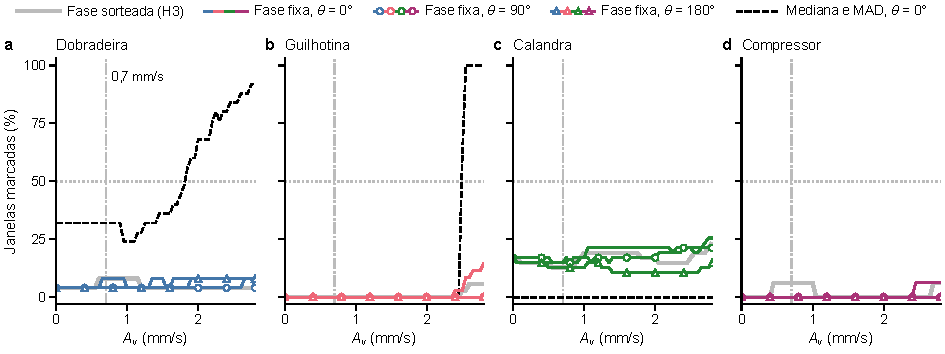
\includegraphics{fig_ap1.pdf}
\fonte{elaborado pelo próprio autor.}
\legenda{fração das janelas de teste marcadas em função da velocidade eficaz $A_v$ da assinatura na rotação, em cada eixo radial, na dobradeira (\textbf{a}), na guilhotina (\textbf{b}), na calandra (\textbf{c}) e no compressor (\textbf{d}). As séries de fase sorteada e de fase fixa são do detector principal. Com a fase sorteada, a de H3, a fase da assinatura variou ao acaso de uma janela para outra; com a fase fixa, $\theta$ é a diferença de fase em relação à componente na rotação de cada eixo. A linha horizontal marca os \SI{50}{\percent} que definem $A_{50}$, e a vertical, o tamanho de referência de \SI{0,7}{\milli\meter\per\second}.}
\end{figure}

\begin{table}[!htb]
\centering\small
\caption{Frações de janelas marcadas com a assinatura em fase fixa com a componente na rotação, na coleta de 2 de novembro de 2026}\label{tab:ap1}
\begin{tabular}{@{}llrrrrrrr@{}}
\toprule
Máquina & Base por eixo & \multicolumn{5}{c}{Detector principal (\%)} & $\Delta d_5$ & MAD \\
\cmidrule(lr){3-7}
 & (mm/s) & Sem & H3 & \SI{0}{\degree} & \SI{90}{\degree} & \SI{180}{\degree} & (mm/s) & (\%) \\
\midrule
Dobradeira & Y \apUmBaseDobradeiraY; Z \apUmBaseDobradeiraZ & \apUmFracaoSemAssinaturaDobradeira & \apUmFracaoSorteadaDobradeira & \apUmFracaoZeroDobradeira & \apUmFracaoNoventaDobradeira & \apUmFracaoCentoOitentaDobradeira & \apUmVariacaoDcincoZeroDobradeira & \apUmMadFracaoZeroDobradeira \\
Guilhotina & X \apUmBaseGuilhotinaX; Z \apUmBaseGuilhotinaZ & \apUmFracaoSemAssinaturaGuilhotina & \apUmFracaoSorteadaGuilhotina & \apUmFracaoZeroGuilhotina & \apUmFracaoNoventaGuilhotina & \apUmFracaoCentoOitentaGuilhotina & \apUmVariacaoDcincoZeroGuilhotina & \apUmMadFracaoZeroGuilhotina \\
Calandra & X \apUmBaseCalandraX; Z \apUmBaseCalandraZ & \apUmFracaoSemAssinaturaCalandra & \apUmFracaoSorteadaCalandra & \apUmFracaoZeroCalandra & \apUmFracaoNoventaCalandra & \apUmFracaoCentoOitentaCalandra & \apUmVariacaoDcincoZeroCalandra & \apUmMadFracaoZeroCalandra \\
Compressor & X \apUmBaseCompressorX; Z \apUmBaseCompressorZ & \apUmFracaoSemAssinaturaCompressor & \apUmFracaoSorteadaCompressor & \apUmFracaoZeroCompressor & \apUmFracaoNoventaCompressor & \apUmFracaoCentoOitentaCompressor & \apUmVariacaoDcincoZeroCompressor & \apUmMadFracaoZeroCompressor \\
\bottomrule
\end{tabular}
\fonte{elaborada pelo próprio autor.}
\nota{a base é a mediana da componente na rotação de cada eixo radial nas janelas de teste sem assinatura. A coluna Sem dá a fração marcada sem assinatura, e a coluna H3, a fração com a fase sorteada de H3; nas colunas \SI{0}{\degree}, \SI{90}{\degree} e \SI{180}{\degree}, $\theta$ é a diferença de fase entre a assinatura e a componente na rotação de cada eixo. $\Delta d_5$ é o aumento médio de $d_5$ nas janelas de teste, e MAD, a fração marcada pela regra por mediana e MAD, as duas com $\theta = \SI{0}{\degree}$. Exceto na coluna Sem, $A_v = \SI{2,8}{\milli\meter\per\second}$. O treino e o teste tiveram \apUmTreinoDobradeira\ e \apUmTesteDobradeira\ janelas na dobradeira, \apUmTreinoGuilhotina\ e \apUmTesteGuilhotina\ na guilhotina, \apUmTreinoCalandra\ e \apUmTesteCalandra\ na calandra e \apUmTreinoCompressor\ e \apUmTesteCompressor\ no compressor.}
\end{table}

Com $\theta = \SI{0}{\degree}$ e \SI{2,8}{\milli\meter\per\second}, a componente $d_5$ das janelas de teste aumentou em média de \apUmVariacaoDcincoZeroDobradeira~mm/s na dobradeira a \apUmVariacaoDcincoZeroGuilhotina~mm/s na guilhotina, enquanto a fração marcada pelo detector principal ficou entre \apUmFracaoZeroCompressor~\% e \apUmFracaoZeroCalandra~\%. Com a mesma injeção, a regra por mediana e MAD chegou a \SI{50}{\percent} de janelas marcadas com \apUmMadAcinquentaZeroDobradeira~mm/s na dobradeira e \apUmMadAcinquentaZeroGuilhotina~mm/s na guilhotina e, com \SI{2,8}{\milli\meter\per\second}, marcou \apUmMadFracaoZeroDobradeira~\% e \apUmMadFracaoZeroGuilhotina~\% das janelas de teste dessas máquinas. Sem assinatura, ela já marcava \apUmMadSemAssinaturaDobradeira~\% das janelas de teste da dobradeira. Na calandra e no compressor, a regra por mediana e MAD não marcou nenhuma janela com $\theta = \SI{0}{\degree}$.

Na dobradeira e na guilhotina, a mudança de $d_5$ produzida pela assinatura em fase bastou para a regra por mediana e MAD e não bastou para o detector principal, treinado com \apUmTreinoDobradeira\ e \apUmTreinoGuilhotina\ janelas. Na calandra e no compressor, nenhum dos dois detectores marcou a assinatura. Em H2, essas duas máquinas tiveram os três ensaios com menor mudança detectável acima de \SI{0,7}{\milli\meter\per\second}. Com a fase fixa, a fração marcada não chegou a \SI{50}{\percent} em nenhuma máquina, e a fase sorteada não explica a refutação de H3.

\subsection{Mediana de várias janelas por medição}\label{sec:res-ap2}

Em H2, cada medição foi uma janela de \SI{0,512}{\second}. Na AP2, a medição passou a ser a mediana de $d_1$ em $k$ janelas consecutivas, com $k$ de 1 a 5, e a menor mudança detectável foi calculada sobre essas medianas como em H2, nos cinco ensaios do critério (Tabela~\ref{tab:ap2}). Janelas consecutivas estavam separadas por \campoCicloUm~s na primeira rodada e por \campoCicloDois~s na segunda, de modo que a mediana de cinco janelas reúne medições espalhadas por quatro desses intervalos. A AP2 não indica o que aconteceria com janelas adquiridas sem intervalo entre elas.

Nos três ensaios em que a menor mudança detectável de uma janela passou de \SI{0,7}{\milli\meter\per\second}, a mediana de até cinco janelas não a levou abaixo desse valor. Nas duas rodadas da calandra, ela diminuiu de \apDoisMmdCalandraUmUm\ e \apDoisMmdCalandraDoisUm~mm/s com uma janela para \apDoisMmdCalandraUmCinco\ e \apDoisMmdCalandraDoisCinco~mm/s com cinco, e no compressor aumentou de \apDoisMmdCompressorUmUm\ para \apDoisMmdCompressorUmCinco~mm/s. Na dobradeira e na segunda rodada da guilhotina, que já ficavam abaixo de \SI{0,7}{\milli\meter\per\second} com uma janela, a menor mudança detectável com cinco janelas foi de \apDoisMmdDobradeiraUmCinco\ e \apDoisMmdGuilhotinaDoisCinco~mm/s.

\begin{table}[!htb]
\centering\small
\caption{Menor mudança detectável no descritor $d_1$ com a mediana de $k$ janelas por medição, na coleta de 2 de novembro de 2026}\label{tab:ap2}
\begin{tabular}{@{}llrrrrrrr@{}}
\toprule
Máquina & Rodada & Janelas & \multicolumn{5}{c}{Menor mudança detectável (mm/s)} & Autocorrelação \\
\cmidrule(lr){4-8}
 & & & $k = 1$ & $k = 2$ & $k = 3$ & $k = 4$ & $k = 5$ & \\
\midrule
Dobradeira & 1 & \hDoisNDobradeiraUm & \apDoisMmdDobradeiraUmUm & \apDoisMmdDobradeiraUmDois & \apDoisMmdDobradeiraUmTres & \apDoisMmdDobradeiraUmQuatro & \apDoisMmdDobradeiraUmCinco & \apDoisAutocorrDobradeiraUm \\
Guilhotina & 2 & \hDoisNGuilhotinaDois & \apDoisMmdGuilhotinaDoisUm & \apDoisMmdGuilhotinaDoisDois & \apDoisMmdGuilhotinaDoisTres & \apDoisMmdGuilhotinaDoisQuatro & \apDoisMmdGuilhotinaDoisCinco & \apDoisAutocorrGuilhotinaDois \\
Calandra & 1 & \hDoisNCalandraUm & \apDoisMmdCalandraUmUm & \apDoisMmdCalandraUmDois & \apDoisMmdCalandraUmTres & \apDoisMmdCalandraUmQuatro & \apDoisMmdCalandraUmCinco & \apDoisAutocorrCalandraUm \\
Calandra & 2 & \hDoisNCalandraDois & \apDoisMmdCalandraDoisUm & \apDoisMmdCalandraDoisDois & \apDoisMmdCalandraDoisTres & \apDoisMmdCalandraDoisQuatro & \apDoisMmdCalandraDoisCinco & \apDoisAutocorrCalandraDois \\
Compressor & 1 & \hDoisNCompressorUm & \apDoisMmdCompressorUmUm & \apDoisMmdCompressorUmDois & \apDoisMmdCompressorUmTres & \apDoisMmdCompressorUmQuatro & \apDoisMmdCompressorUmCinco & \apDoisAutocorrCompressorUm \\
\bottomrule
\end{tabular}
\fonte{elaborada pelo próprio autor.}
\nota{com $k$ janelas, a medição é a mediana móvel de $d_1$ em $k$ janelas consecutivas, com passo de uma janela, e a menor mudança detectável é calculada sobre essas medianas como em H2; com $k = 1$, ela é a da Tabela~\ref{tab:h2}. A autocorrelação é a correlação de Pearson entre os valores de $d_1$ de janelas consecutivas.}
\end{table}

O compressor foi o único ensaio com autocorrelação positiva de $d_1$ entre janelas consecutivas, de \apDoisAutocorrCompressorUm. Com autocorrelação positiva, janelas vizinhas variam juntas, e a mediana delas reduz pouco a variação, o que é compatível com o aumento da menor mudança detectável no compressor. Nos outros quatro ensaios, a autocorrelação foi de \apDoisAutocorrDobradeiraUm\ a \apDoisAutocorrGuilhotinaDois.

Em dois ensaios, a menor mudança detectável não diminuiu de forma monotônica com $k$. Na segunda rodada da guilhotina, ela aumentou para \apDoisMmdGuilhotinaDoisDois~mm/s com duas janelas e diminuiu para \apDoisMmdGuilhotinaDoisTres~mm/s com três. A mediana de duas janelas é a média delas e mantém metade de um valor alto isolado, que a de três janelas descarta, e essa diminuição é compatível com valores altos em janelas isoladas. Na segunda rodada da calandra, a menor mudança detectável oscilou entre \apDoisMmdCalandraDoisQuatro\ e \apDoisMmdCalandraDoisTres~mm/s de $k = 2$ a $k = 5$. Como medianas vizinhas compartilham janelas, o quantil de \SI{95}{\percent} da série depende de poucos valores altos.

\subsection{Falso alarme com outras sementes e com o treino reamostrado}\label{sec:res-ap3}

O limiar e o modelo de H1 e de H4 foram estimados uma vez, com a semente 0 do gerador de números aleatórios do Isolation Forest, e o intervalo registrado reamostra só as janelas de teste. A AP3 mediu a variação que esse intervalo não inclui de duas formas. Na primeira, o detector foi treinado com as sementes de 0 a \num{99}, cada uma com o seu limiar, sobre o mesmo treino e o mesmo teste. Na segunda, em \apTresReplicas\ réplicas, o treino foi reamostrado por blocos de cinco janelas consecutivas, e o limiar e o modelo foram refeitos com uma semente diferente em cada réplica, antes da reamostragem do teste. Na validação do limiar, todas as cópias de um mesmo bloco ficaram no mesmo grupo, para que nenhuma janela recebesse escore de um modelo treinado com ela. Na calandra, \apTresDescartesCalandra\ das \apTresReplicas\ réplicas teve um só bloco distinto no treino, sem como validar o limiar, e foi descartada, caso que o registro não previa. A segunda forma não se aplica à guilhotina, cujo treino de \campoJanelasGuilhotinaUm\ janelas tem só três blocos.

Na calandra, a fração marcada na segunda rodada teve mediana de \apTresSementeCalandraMed~\% entre as \apTresSementes\ sementes, com \SI{95}{\percent} delas de \apTresSementeCalandraPInf~\% a \apTresSementeCalandraPSup~\% e extremos de \apTresSementeCalandraMin~\% e \apTresSementeCalandraMax~\% (Tabela~\ref{tab:ap3}). A semente 0, registrada, deu \hUmFracaoCalandra~\%, acima da mediana. A fração ficou em até \SI{10}{\percent} com \apTresSementeCalandraAteDez\ sementes e passou de \SI{20}{\percent} com \apTresSementeCalandraAcimaVinte. Com o treino reamostrado, o intervalo foi de \apTresTreinoInfCalandra~\% a \apTresTreinoSupCalandra~\%, mais largo que o registrado, de \hUmCalandraIFDiretoInf~\% a \hUmCalandraIFDiretoSup~\%. Na guilhotina, nenhuma das \apTresSementes\ florestas, treinadas com as \campoJanelasGuilhotinaUm\ janelas da primeira rodada, marcou janela da segunda.

Pelos critérios registrados, aplicados a cada semente com o intervalo do teste reamostrado, H1 seria corroborada com \apTresVereditoUmCorroborada\ sementes, indeterminada com \apTresVereditoUmIndeterminada\ e refutada com \apTresVereditoUmRefutada. O veredito de H1 depende, portanto, da semente do detector, e o veredito registrado, calculado com a semente 0, continua valendo.

Em H4, o falso alarme em 0E teve mediana de \apTresSementeNivelZeroMed~\% entre as sementes, com \SI{95}{\percent} delas de \apTresSementeNivelZeroPInf~\% a \apTresSementeNivelZeroPSup~\%. O número de sementes com falso alarme acima de \SI{20}{\percent} foi \apTresSementeNivelZeroAcimaVinte, e o de sementes com até \SI{10}{\percent}, \apTresSementeNivelZeroAteDez. A fração marcada chegou a \SI{50}{\percent} nos quatro níveis de desbalanceamento ao mesmo tempo com \apTresSementeNiveisCinquenta\ sementes. Com o treino reamostrado, o intervalo do falso alarme foi de \apTresTreinoInfNivelZero~\% a \apTresTreinoSupNivelZero~\%. Pelos critérios registrados, H4 seria refutada com \apTresVereditoQuatroRefutada\ sementes e indeterminada com \apTresVereditoQuatroIndeterminada, e o número de sementes que a corroborariam foi \apTresVereditoQuatroCorroborada. A refutação de H4 não depende, portanto, da semente.

Com o treino reamostrado, a fração marcada nos níveis 2 a 4 também foi de quase nenhuma janela a todas, e em \descReplicasSemMarcacaoQuatro\ das \apTresReplicas\ réplicas nenhuma janela de 4E, o nível de maior desbalanceamento, passou do limiar. Para descrever esse resultado, o modelo registrado de H4 foi aplicado de novo às janelas de cada arquivo, numa descrição acrescentada depois do cálculo e fora do registro. As janelas de 4E tinham, em mediana, \descForaMedianaQuatro\ descritores fora da faixa do treino, e o escore delas ficou entre \descEscoreCincoPctQuatro, no percentil de \SI{5}{\percent}, e \descEscoreMaxQuatro, no máximo, pouco acima do limiar registrado, de \descLimiarQuatro. O escore das janelas de maior desbalanceamento ficou, assim, numa faixa estreita, compatível com o teto do escore fora da faixa do treino (seção~\ref{sec:res-ap6}). Com outro treino e outro limiar, essa faixa pode ficar toda abaixo do limiar, como nas réplicas sem nenhuma janela marcada.

\begin{table}[!htb]
\centering\small
\caption{Fração de janelas marcadas com as sementes de 0 a 99 e com o treino reamostrado}\label{tab:ap3}
\setlength{\tabcolsep}{4pt}
\begin{tabular}{@{}llrrrrr@{}}
\toprule
Hipótese & Teste & Semente 0 & \multicolumn{3}{c}{Sementes de 0 a \num{99} (\%)} & Treino \\
\cmidrule(lr){4-6}
 & & (\%) & Mediana & \SI{95}{\percent} das sementes & Extremos & reamostrado (\%) \\
\midrule
H1, calandra & rodada 2 & \hUmFracaoCalandra & \apTresSementeCalandraMed & \apTresSementeCalandraPInf\ a \apTresSementeCalandraPSup & \apTresSementeCalandraMin\ a \apTresSementeCalandraMax & \apTresTreinoInfCalandra\ a \apTresTreinoSupCalandra \\
H1, guilhotina & rodada 2 & \hUmFracaoGuilhotina & \apTresSementeGuilhotinaMed & \apTresSementeGuilhotinaPInf\ a \apTresSementeGuilhotinaPSup & \apTresSementeGuilhotinaMin\ a \apTresSementeGuilhotinaMax & \\
H4 & 0E & \hQuatroFracaoZero & \apTresSementeNivelZeroMed & \apTresSementeNivelZeroPInf\ a \apTresSementeNivelZeroPSup & \apTresSementeNivelZeroMin\ a \apTresSementeNivelZeroMax & \apTresTreinoInfNivelZero\ a \apTresTreinoSupNivelZero \\
H4 & 1E & \hQuatroFracaoUm & \apTresSementeNivelUmMed & \apTresSementeNivelUmPInf\ a \apTresSementeNivelUmPSup & \apTresSementeNivelUmMin\ a \apTresSementeNivelUmMax & \apTresTreinoInfNivelUm\ a \apTresTreinoSupNivelUm \\
H4 & 2E & \hQuatroFracaoDois & \apTresSementeNivelDoisMed & \apTresSementeNivelDoisPInf\ a \apTresSementeNivelDoisPSup & \apTresSementeNivelDoisMin\ a \apTresSementeNivelDoisMax & \apTresTreinoInfNivelDois\ a \apTresTreinoSupNivelDois \\
H4 & 3E & \hQuatroFracaoTres & \apTresSementeNivelTresMed & \apTresSementeNivelTresPInf\ a \apTresSementeNivelTresPSup & \apTresSementeNivelTresMin\ a \apTresSementeNivelTresMax & \apTresTreinoInfNivelTres\ a \apTresTreinoSupNivelTres \\
H4 & 4E & \hQuatroFracaoQuatro & \apTresSementeNivelQuatroMed & \apTresSementeNivelQuatroPInf\ a \apTresSementeNivelQuatroPSup & \apTresSementeNivelQuatroMin\ a \apTresSementeNivelQuatroMax & \apTresTreinoInfNivelQuatro\ a \apTresTreinoSupNivelQuatro \\
\bottomrule
\end{tabular}
\fonte{elaborada pelo próprio autor, com dados de \citeonline{mey2022dados} nas linhas de H4.}
\nota{semente 0: valor registrado. Nas sementes de 0 a \num{99}, cada floresta tem o seu limiar, com o mesmo treino e o mesmo teste; \SI{95}{\percent} das sementes vai do percentil de \SI{2,5}{\percent} ao de \SI{97,5}{\percent}. Treino reamostrado: intervalo de \SI{95}{\percent} de \apTresReplicas\ réplicas, com treino e teste reamostrados por blocos e limiar e modelo refeitos em cada réplica; não calculado na guilhotina, cujo treino tem três blocos. Em H1, o teste é a segunda rodada; em H4, 0E não tem desbalanceamento, e 1E a 4E têm os níveis 1 a 4.}
\end{table}

\subsection{Intervalo da menor mudança detectável}\label{sec:res-ap4}

A menor mudança detectável de H2 é a diferença entre o quantil de \SI{95}{\percent} e a mediana de $d_1$, e o quantil de \SI{95}{\percent} de \num{25} a \num{50} janelas depende das duas ou três janelas mais altas. Na AP4, as janelas de cada ensaio foram reamostradas por blocos de cinco janelas consecutivas, em \num{2000} réplicas, e a menor mudança detectável foi recalculada em cada réplica (Tabela~\ref{tab:ap4}).

\begin{table}[!htb]
\centering\small
\caption{Intervalo da menor mudança detectável no descritor $d_1$ e comparação com o sensor em repouso, na coleta de 2 de novembro de 2026}\label{tab:ap4}
\setlength{\tabcolsep}{4pt}
\begin{tabular}{@{}llrrrr@{}}
\toprule
Ensaio & Rodada & \multicolumn{2}{c}{Menor mudança detectável (mm/s)} & Réplicas acima & Razão com \\
\cmidrule(lr){3-4}
 & & Amostra & Intervalo de \SI{95}{\percent} & de \SI{0,7}{\milli\meter\per\second} (\%) & o repouso \\
\midrule
Dobradeira & 1 & \hDoisMmdDobradeiraUm & \apQuatroInfDobradeiraUm\ a \apQuatroSupDobradeiraUm & \apQuatroAcimaDobradeiraUm & \apCincoRazaoDobradeiraUm \\
Guilhotina & 1 & \hDoisMmdGuilhotinaUm & \apQuatroInfGuilhotinaUm\ a \apQuatroSupGuilhotinaUm & \apQuatroAcimaGuilhotinaUm & \\
Guilhotina & 2 & \hDoisMmdGuilhotinaDois & \apQuatroInfGuilhotinaDois\ a \apQuatroSupGuilhotinaDois & \apQuatroAcimaGuilhotinaDois & \apCincoRazaoGuilhotinaDois \\
Calandra & 1 & \hDoisMmdCalandraUm & \apQuatroInfCalandraUm\ a \apQuatroSupCalandraUm & \apQuatroAcimaCalandraUm & \apCincoRazaoCalandraUm \\
Calandra & 2 & \hDoisMmdCalandraDois & \apQuatroInfCalandraDois\ a \apQuatroSupCalandraDois & \apQuatroAcimaCalandraDois & \apCincoRazaoCalandraDois \\
Compressor & 1 & \hDoisMmdCompressorUm & \apQuatroInfCompressorUm\ a \apQuatroSupCompressorUm & \apQuatroAcimaCompressorUm & \apCincoRazaoCompressorUm \\
\midrule
Repouso & & \apCincoMmd & \apCincoMmdInf\ a \apCincoMmdSup & & \\
Repouso, X e Y & & \apCincoMmdHorizontal & \apCincoMmdInfHorizontal\ a \apCincoMmdSupHorizontal & & \\
\bottomrule
\end{tabular}
\fonte{elaborada pelo próprio autor.}
\nota{intervalo pelos percentis de \SI{2,5}{\percent} e \SI{97,5}{\percent} de \num{2000} réplicas, com reamostragem por blocos de cinco janelas consecutivas. A razão com o repouso divide a menor mudança detectável do ensaio pela do sensor em repouso, de \apCincoMmd~mm/s, calculada pela mesma regra nas \apCincoJanelas\ janelas com o transmissor sobre a mesa; a primeira rodada da guilhotina, fora do critério de H2, não tem razão calculada. Na linha Repouso, X e Y, $d_1$ é o maior valor entre os eixos horizontais X e Y.}
\end{table}

Nas duas rodadas da calandra e no compressor, todas as réplicas ficaram acima de \SI{0,7}{\milli\meter\per\second}, e o limite inferior do intervalo foi de \apQuatroInfCompressorUm~mm/s no compressor a \apQuatroInfCalandraDois~mm/s na segunda rodada da calandra. Na dobradeira, nenhuma réplica chegou a \SI{0,7}{\milli\meter\per\second}, e o intervalo foi de \apQuatroInfDobradeiraUm\ a \apQuatroSupDobradeiraUm~mm/s. Na segunda rodada da guilhotina, o intervalo foi de \apQuatroInfGuilhotinaDois\ a \apQuatroSupGuilhotinaDois~mm/s, e \apQuatroAcimaGuilhotinaDois~\% das réplicas passaram de \SI{0,7}{\milli\meter\per\second}. A largura desse intervalo se deve a poucas janelas com $d_1$ alto, que entram em parte das réplicas e ficam fora de outras. Com amostras desse tamanho, a reamostragem de quantis extremos tende a dar intervalos estreitos demais, e os intervalos da Tabela~\ref{tab:ap4} são aproximados.

\subsection{Menor mudança detectável com o sensor em repouso}\label{sec:res-ap5}

A comparação com o ruído usa, na AP5, a mesma regra de H2 aplicada às \apCincoJanelas\ janelas com o transmissor parado sobre a mesa. Nessas janelas, a mediana de $d_1$ foi de \apCincoMediana~mm/s, e a menor mudança detectável, de \apCincoMmd~mm/s, com intervalo de \apCincoMmdInf\ a \apCincoMmdSup~mm/s (Tabela~\ref{tab:ap4}). Só com os eixos horizontais, X e Y, sem o eixo vertical, que tem linhas compatíveis com a vibração da mesa (seção~\ref{sec:res-aquisicao}), a menor mudança detectável em repouso foi de \apCincoMmdHorizontal~mm/s.

Nos cinco ensaios do critério de H2, a menor mudança detectável ficou de \apCincoRazaoMin\ a \apCincoRazaoMax\ vezes a do repouso, e de \apCincoRazaoHorizontalMin\ a \apCincoRazaoHorizontalMax\ vezes a do repouso só nos eixos horizontais. As duas razões passam de 1 em todos os ensaios, e a variação de $d_1$ entre janelas nas máquinas foi maior que a do mesmo descritor com o sensor parado. A razão não separa a máquina da fixação, porque o sinal das máquinas inclui as duas e o do repouso não inclui nenhuma.

\subsection{Escore do detector fora da faixa do treino}\label{sec:res-ap6}

Em cada árvore do Isolation Forest, o valor da divisão de um nó é sorteado entre o mínimo e o máximo das janelas desse nó. Uma janela além do máximo do treino num descritor segue o mesmo caminho em qualquer distância além dele, e o escore deixa de crescer com a distância. Na AP6, o escore foi calculado em pontos sintéticos com a mediana do treino em cada descritor, exceto nos descritores deslocados para além da faixa do treino, e comparado com o limiar de cada modelo (Tabela~\ref{tab:ap6}). Antes do cálculo, o escore de cada ponto foi conferido com o dobro da distância além da faixa, e não mudou.

\begin{table}[!htb]
\centering\small
\caption{Escore do detector principal em pontos fora da faixa do treino}\label{tab:ap6}
\begin{tabular}{@{}lrrrrrr@{}}
\toprule
Modelo & Treino & Limiar & Referência & Um descritor & $d_1$, $d_2$ e $d_5$ & Seis descritores \\
 & (janelas) & & & fora (maior) & fora & fora \\
\midrule
Dobradeira & \apSeisTreinoDobradeira & \apSeisLimiarDobradeira & \apSeisReferenciaDobradeira & \apSeisUmMaxDobradeira & \apSeisTresDobradeira & \apSeisTodosDobradeira \\
Guilhotina & \apSeisTreinoGuilhotina & \apSeisLimiarGuilhotina & \apSeisReferenciaGuilhotina & \apSeisUmMaxGuilhotina & \apSeisTresGuilhotina & \apSeisTodosGuilhotina \\
Calandra & \apSeisTreinoCalandra & \apSeisLimiarCalandra & \apSeisReferenciaCalandra & \apSeisUmMaxCalandra & \apSeisTresCalandra & \apSeisTodosCalandra \\
Compressor & \apSeisTreinoCompressor & \apSeisLimiarCompressor & \apSeisReferenciaCompressor & \apSeisUmMaxCompressor & \apSeisTresCompressor & \apSeisTodosCompressor \\
Base pública & \hQuatroNTreino & \apSeisLimiarQuatro & \apSeisReferenciaQuatro & \apSeisUmMaxQuatro & \apSeisTresQuatro & \apSeisTodosQuatro \\
\bottomrule
\end{tabular}
\fonte{elaborada pelo próprio autor, com dados de \citeonline{mey2022dados} na última linha.}
\nota{escore do detector principal com a semente 0, nos modelos de H3 (os da guilhotina e da calandra são também os de H1) e no de H4. Referência: ponto com a mediana do treino nos seis descritores. Fora: descritor colocado além do máximo do treino, ou abaixo do mínimo na coluna de um descritor, que dá o maior escore entre os doze pontos com um só descritor deslocado. Os demais descritores ficam na mediana do treino.}
\end{table}

Com um só descritor fora da faixa, o escore ficou abaixo do limiar nos cinco modelos, em qualquer direção e em qualquer distância. Com $d_1$, $d_2$ e $d_5$ fora da faixa, os três descritores que a assinatura de H3 aumenta, o escore passou do limiar só no modelo da dobradeira, com \apSeisTresDobradeira\ contra \apSeisLimiarDobradeira, e ficou abaixo dele nos modelos da guilhotina, da calandra, do compressor e da base pública. Nesses quatro modelos, uma janela que mude só esses três descritores, com os demais perto da mediana do treino, não alcança o limiar em nenhuma amplitude. Com os seis descritores fora, o escore passou do limiar em todos os modelos.

Na injeção de H3, a mediana de $d_5$ das janelas de teste passou do máximo do treino com \apSeisAsatGuilhotina~mm/s na guilhotina, \apSeisAsatDobradeira~mm/s na dobradeira e \apSeisAsatCompressor~mm/s no compressor, e na calandra não passou até \SI{2,8}{\milli\meter\per\second}. Com \SI{2,8}{\milli\meter\per\second}, \apSeisJanelasDcincoAcimaGuilhotina\ das \apSeisTesteGuilhotina\ janelas de teste da guilhotina estavam com $d_5$ acima do máximo do treino, e a mediana do escore foi de \apSeisEscoreAltoGuilhotina, abaixo do limiar de \apSeisLimiarGuilhotina. Pela leitura registrada, a refutação de H3 na guilhotina e no compressor se deve ao escore máximo do detector com o treino de cada máquina, e não à amplitude da assinatura. Na calandra, o escore máximo com os três descritores fora também fica abaixo do limiar, mas a assinatura de \SI{2,8}{\milli\meter\per\second} não chegou a levar a mediana de $d_5$ além da faixa do treino, porque a componente já presente tinha mediana de \hTresBaseUmXCalandra~mm/s.
